% Many thanks to Andrew West for writing most of this file
% Main LaTeX file for CIS400/401 Project Proposal Specification
%
% Once built and in PDF form this document outlines the format of a
% project proposal. However, in raw (.tex) form, we also try to
% comment on some basic LaTeX technique. This is not intended to be a
% LaTeX tutorial, instead just (1) a use-case thereof, and (2) a
% template for your own writing.

% Ordinarily we'd begin by specifying some broad document properties
% like font-size, page-size, margins, etc. -- We have done this (and
% much more) for you by creating a 'style file', which the
% 'documentclass' command references.
\documentclass{sig-alternate}
 
% These 'usepackage' commands are a way of importing additional LaTeX
% styles and formattings that aren't part of the 'standard library'
\usepackage{mdwlist}
\usepackage{url}
\usepackage{tabularx}
\usepackage{tikz}
\usetikzlibrary{shapes,arrows}
\usepackage[export]{adjustbox}
\usepackage{lipsum,adjustbox}
\usepackage{listings}% http://ctan.org/pkg/listings
\lstset{
  basicstyle=\ttfamily,
  mathescape
}\begin{document} 

% We setup the parameters to our title header before 'making' it. Note
% that your proposals should have actual titles, not the generic one
% we have here.
\title{Verification of System FC in Coq}
\subtitle{Dept. of CIS - Senior Design 2014-2015\thanks{Advisors: Stephanie Weirich (sweirich@cis.upenn.edu), Richard Eisenberg (eir@cis.upenn.edu).}}
\numberofauthors{4}
\author{
  Tiernan Garsys \\ \email{tgarsys@seas.upenn.edu} \\ Univ. of Pennsylvania \\ Philadelphia, PA\\\\
  Lucas Pe\~{n}a \\ \email{lpena@seas.upenn.edu} \\ Univ. of Pennsylvania \\ Philadelphia, PA
  \and
  Tayler Mandel \\ \email{tmandel@seas.upenn.edu} \\ Univ. of Pennsylvania \\ Philadelphia, PA\\\\
  Noam Zilberstein \\ \email{noamz@seas.upenn.edu} \\ Univ. of Pennsylvania \\ Philadelphia, PA
}
\date{}
\maketitle

% Next we write out our abstract -- generally a two paragraph maximum,
% executive summary of the motivation and contributions of the work.
\begin{abstract}
  \textit{
Haskell's compiler, the Glasgow Haskell Compiler (GHC), generates code in GHC Core. The Coq proof assistant will be used to verify a formalized version of System FC, the basis for GHC Core. A translation from the formal language to GHC Core, the concrete implementation of System FC that is used in GHC, will then be proven. The goal of verification is to prove that the evaluation semantics of System FC are sound.
  }

  \textit{
There are two main benefits to this project. First, the verification would provide assurance regarding the safety and accuracy of GHC. Second, and perhaps more importantly, it will provide foundation to verify other properties of GHC such as compiler optimizations.
 }
\end{abstract}

% Then we proceed into the body of the report itself. The effect of
% the 'section' command is obvious, but also notice 'label'. Its good
% practice to label every (sub)-section, graph, equation etc. -- this
% gives us a way to dynamically reference it later in the text via the
% 'ref' command, e.g., instead of writing `Section 1', you can write
% `Section~\ref{sec:intro}', which is useful if the section number
% changes.
\section{Introduction}
\label{sec:intro}
Haskell has one of the strongest type systems of any mainstream programming language with features such as type families, typeclasses, and generalized algebraic datatypes (datatypes that have non-standard constructors). When writing Haskell, there are many guarantees of correctness encoded in the type system. Ensuring that the type safety of features like these is preserved in Haskell would be greatly beneficial as it would act as a proof of correctness for the language.

The Glasgow Haskell Compiler (GHC) is used to compile Haskell code into native executables. The entire GHC compilation process is outlined in Figure~\ref{fig:desgar}. First, Haskell code is typechecked and then desugared to obtain code in an intermediate language called GHC-Core. The desugaring process removes specialized syntax that is helpful for programmers. A core language, such as GHC-Core, is the result of a translation from a surface language, such as Haskell, to a language that a compiler can better reason about. Whereas types are important in programming languages to prevent a user from making errors, types are important in core languages to prevent the compiler from making errors. GHC Core is an implementation of a language specification called System FC. A first step in proving the type safety of Haskell is proving the type safety of System FC. This type safety is ensured by proving the progress, preservation, and soundness theorems using the formalized definition of System FC.

\begin{figure}[h!]
  \centering
  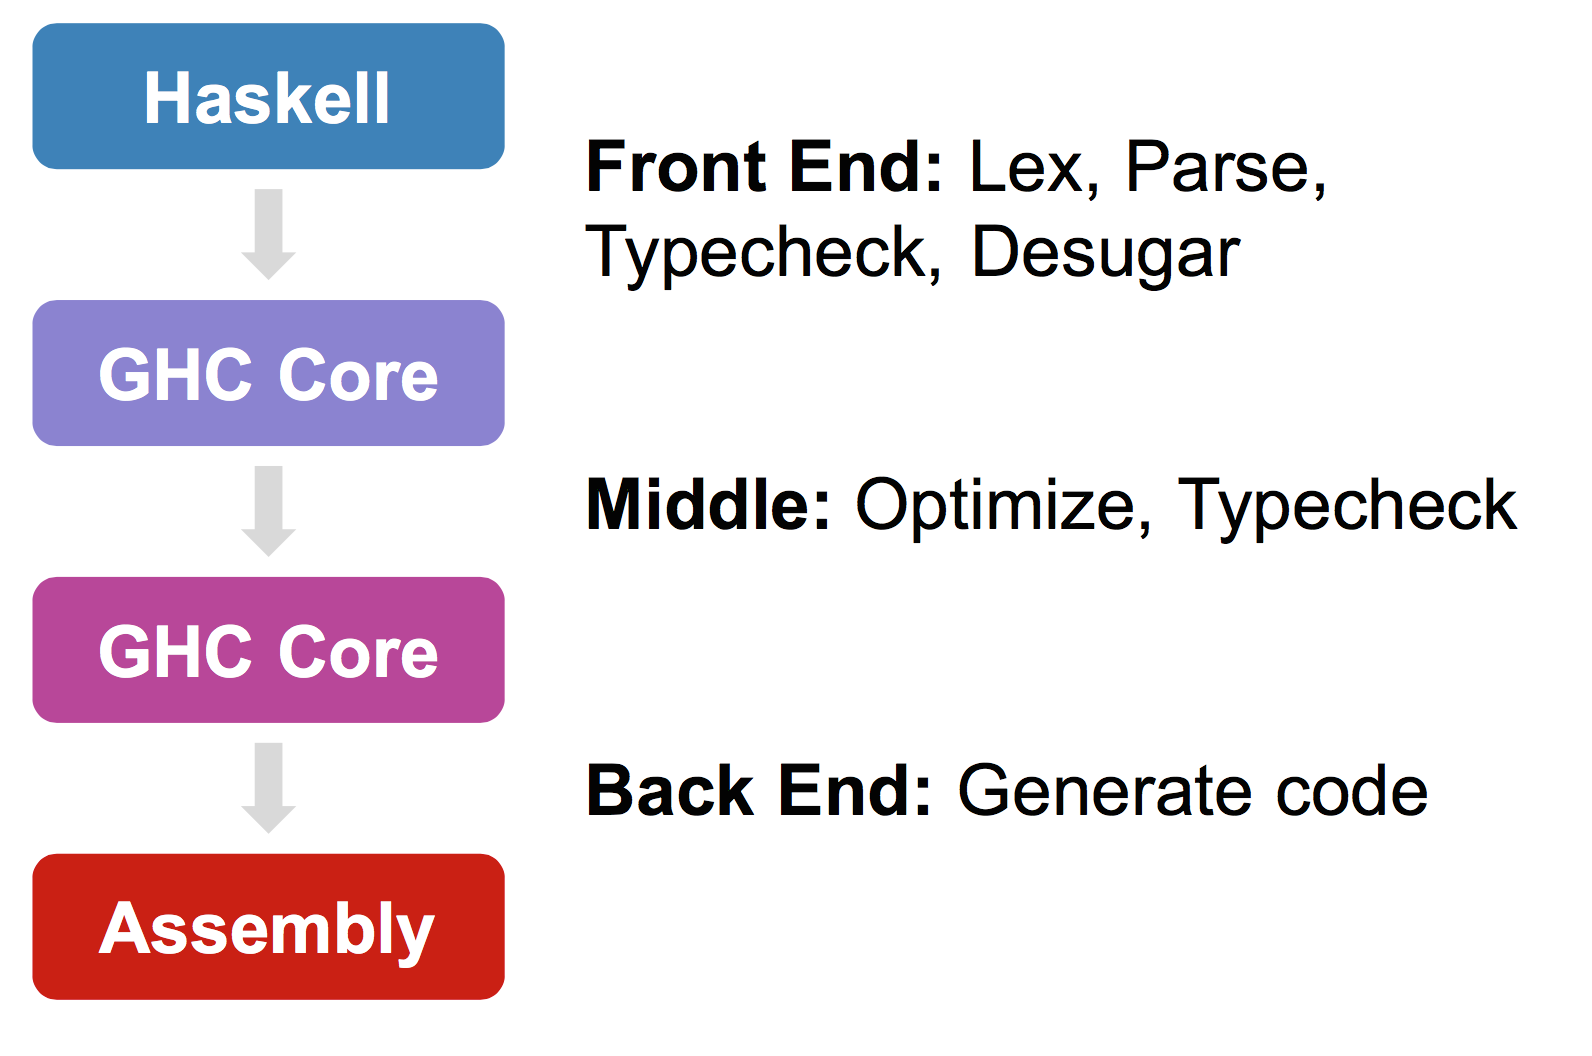
\includegraphics[max width=3in]{desgar.png}
  \caption{The GHC compilation process}
  \label{fig:desgar}
\end{figure}

There is no formal proof that GHC Core is type safe. Formally verifying System FC allows for future work in the formal verification of GHC. Once the core language is verified, it becomes possible to verify that transformations of this core language preserve the typing and progression semantics of the original language~\cite{zhao2013formalizing}. One particularly relevant class of transformations on the core language is the set of compiler optimizations performed by GHC. While these transformations can improve the runtime of one's code, they can also introduce bugs due to the semantics of the original code not being preserved under the optimization. With the semantics of the source language formalized and verified, it becomes easy to extend the formalizations to encompass the changes made under these optimizations, and thus verify their correctness~\cite{Zhao:2012:FLI:2103656.2103709}. Another major use is the ability to extend the proof, in order to verify extensions to System FC. Such extensions to System FC are used to add new features to the surface language.

To accomplish this, GHC Core is verified in a series of steps. First, System F, the foundation upon which System FC is built, is verified. Coercions, type families, and datatypes are then added to bring this formalization System F up to feature parity with System FC. 

\section{Background}
\label{sec:background}
In order to understand the goals of verification, it is necessary to define some background concepts and terminology. In Section~\ref{sec:prog-pres}, the idea of language semantics and what it means for a language to be type safe is defined. This idea of type safety is defined as the union of two theorems: Progress and Preservation. If these two theorems are proven given the specification of a language such as System F, then the language is considered to be type safe. In Section~\ref{sec:system-f}, the specific semantics of System F are provided. Next, the features that appear in System FC but are absent from System F are defined. These features are coercions (Section~\ref{sec:coercions}), type families (Section~\ref{sec:type-fam}), and datatypes (Section~\ref{sec:datatypes}).

\subsection{Progress and Preservation}
\label{sec:prog-pres}
Progress, preservation, and soundness are the most basic indications of safety for any type system~\cite{Pierce:TAPL}. To understand these, it is important to define how the operational semantics of a language are formalized. Types are descriptors for data and terms are well-typed expressions under a given context, or set of typing assumptions. When specifying the operational semantics of a programming language, one defines a step relation that relates a term of a particular type in the language to another term of the same type. Terms make steps in order to reach a simplified form (see Figure~\ref{fig:step-ex} for an example). The evaluation of any expression in the language can be modeled in a series of discrete ``steps'', where in each step one takes a term in the expression and replaces it with the resulting term per the step relation. In a well-typed program, this process continues until the expression evaluates to a value, a unique representation of a term for a particular type that cannot be evaluated further via the step relation (e.g. `true' or 'false' for the type of booleans).

\begin{figure}[h!]
  $$(\lambda x .\; \lambda y .\;x+y)\; 3 \rightarrow \lambda y.\;3+y$$
  \caption{Concrete example of a the step relation for a function application, known formally as Beta Reduction}
  \label{fig:step-ex}
\end{figure}

The progress, preservation, and soundness theorems can now be defined. Progress states that a well-typed term is either a value, or can take a step per the step relation. Preservation indicates that if a well-typed term takes a step, the resulting term will still be well-typed. If something cannot take a step and is not a value, the program is said to be stuck. Combining these definitions, soundness states that a well typed program will never become stuck~\cite{Pierce:TAPL}. This stuckness will cause errors including but not limited to a segmentation fault. \\\\\\
\noindent\textbf{Theorem (Progress)} \textit{For all terms $t$, types $T$, and contexts $\Gamma$, if $t$ has type $T$ under context $\Gamma$ then either $t$ is a value, or there exists a term $t'$ such that $t$ steps to $t'$} \\

\noindent\textbf{Theorem (Preservation)} \textit{For all terms $t$ and $t'$, types $T$, and contexts $\Gamma$, if $t$ has type $T$ under the context $\Gamma$ and $t$ steps to $t'$ then $t'$ has type $T$ under the context $\Gamma$.} \\

\noindent\textbf{Theorem (Soundness)} \textit{Any well-typed program will never reach a stuck state during evaluation.}

\newcommand\mybox[2][]{#2}%\tikz[overlay]\node[fill=white!20,inner sep=2pt, anchor=text, rectangle, rounded corners=1mm,#1] {#2};\phantom{#2}}
\begin{figure}[h!]
  \noindent{\large\it Syntax}\\
  \begin{tabular}{l l r}
    \hline
    $t$ ::= && \textbf{ Terms:}\\
    & $x$ & \textit{variable}\\
    & $\lambda x:T.t$ & \textit{abstraction}\\
    & $t\; t$ & \textit{application}\\
    & \mybox[fill=blue!20]{$\lambda X.t$} & \textit{type abstraction}\\
    & \mybox[fill=blue!20]{$t\; [T]$} & \textit{type application}\\
    \hspace{.3in} & \hspace{1.3in} & \hspace{2.1in}\\
    $v$ ::= && \textbf{Values:}\\
    & $\lambda x:T.t$ & \textit{abstraction value}\\
    & \mybox[fill=blue!20]{$\lambda X.t$} & \textit{type abstraction value}\\\\
    $T$ ::= && \textbf{Types:}\\
    & \mybox[fill=blue!20]{$X$} & \textit{type variable}\\
    & $T\rightarrow T$ & \textit{type of functions}\\
    & \mybox[fill=blue!20]{$\forall X.T$} & \textit{universal type}\\\\
    $\Gamma$ ::= && \textbf{Contexts:}\\
    & $\varnothing$ & \textit{empty context}\\
    & $\Gamma,x:T$ & \textit{term variable binding}\\
    & \mybox[fill=blue!20]{$\Gamma,X$} & \textit{type variable binding}\\
  \end{tabular}
  \caption{Syntax for System F}
  \label{fig:syntax}
\end{figure}

\begin{figure}[h!]
  \noindent{\large\it Evaluation}\\
  \begin{tabular}{c r}
    \hline
    $t_1\rightarrow t_1$\\$\overline{t'_1\; t_2\rightarrow t'_1\; t_2}$ & (E-App1)\\\\
    $t_2\rightarrow t'_2$\\$\overline{v_1\; t_2\rightarrow v_1\; t'_2}$ & (E-App2)\\\\
    $(\lambda x:T_{11}.t_{12})\; v_2\rightarrow[x\mapsto v_2]t_{12}$ & (E-AppAbs)\\\\
    \mybox[fill=blue!20]{$t_1\rightarrow t'_1$}\\\mybox[fill=blue!20]{$\overline{t_1\; [T_2]\rightarrow t'_1\; [T_2]}$} & (E-TApp)\\\\
    \mybox[fill=blue!20]{$(\lambda X.t_{12})\; [T_2]\rightarrow [X\mapsto T_2]t_{12}$} & (E-TAppTAbs)\\
    \hspace{2in} & \hspace{1in}
  \end{tabular}
  \caption{Evaluation semantics for System F}
  \label{fig:evaluation}
\end{figure}

\begin{figure}[h!]
  {\large\it Typing}\\
  \begin{tabular}{c r}
    \hline
    $x:T\in\Gamma$\\$\overline{\Gamma\vdash x:T}$ & (T-Var)\\\\
    $\Gamma, x:T_1\vdash t_2:T_2$\\$\overline{\Gamma\vdash\lambda x:T_1.t_2\; :\; T_1\rightarrow T_2}$ & (T-Abs)\\\\
    $\underline{\Gamma\vdash t_1 : T_{11}\rightarrow T_{12}\; \; \; \; \; \; \; \; \Gamma\vdash t_2 : T_{11}}$\\$\Gamma\vdash t_1\; t_2 : T_{12}$ & (T-App)\\\\
    \mybox[fill=blue!20]{$\Gamma,X\vdash t_2 : T_2$}\\\mybox[fill=blue!20]{$\overline{\Gamma\vdash\lambda X.t_2 : \forall X.T_2}$} & (T-TAbs)\\\\
    \mybox[fill=blue!20]{$\Gamma\vdash t_1 : \forall X.T_{12}$}\\\mybox[fill=blue!20]{$\overline{\Gamma\vdash t_1\; [T_2] : [X\mapsto T_2]T_{12}}$} & (T-TApp)\\
    \hspace{2in} & \hspace{1in}
  \end{tabular}
  \caption{Typing relations for System F}
  \label{fig:typing}
\end{figure}

Together, these properties guarantee that a well-typed program in the specified language will always be able to continue evaluation until it reaches a value; the result of the program ending up in a stuck state will only result from the program logic leading to an infinite loop, and not from the language falling into some invalid state. After formalizing the operational semantics for System FC, it is demonstrated that preservation, progress, and soundness hold for the specification.

\subsection{System F}
\label{sec:system-f}
System FC is built on top of the simpler language System F. System F, also known as the polymorphic lambda calculus, is an extension of the simply-typed lambda calculus to include the abstraction and application of types~\cite{Pierce:TAPL}. This feature essentially allows for functions to take types as parameters, granting the ability to define functions whose actual types vary based on these input types. The syntax for System F is provided in Figure~\ref{fig:syntax}, the evaluation semantics are outlined in Figure~\ref{fig:evaluation}, and type relations are stated in Figure~\ref{fig:typing}. System F is formalized in Coq and then additional features are added in order to transform System F into a full formalization of System FC. These features include type coercion, type families, and datatypes. Using System F as a base language, a proof of System FC is formalized, and a translation from System FC to GHC Core is then proven which shows that the core language of GHC has indeed been verified. 

\subsection{Coercions}
\label{sec:coercions}
Coercions are responsible for most of the power of System FC over System F. They allow a conversion from one type to another. In particular, type coercions allow for type families and generalized algebraic datatypes to exist in System FC by acting as a witness for equality between syntactically different types~\cite{DBLP:conf/rta/VytiniotisJ13}. Types can be equal in different ways and therefore there is a complex set of coercion rules that can be used to construct correct equality proofs~\cite{Breitner:2014:SZC:2628136.2628141}. A basic example of the usefulness of coercions is provided in Figures~\ref{fig:coercion-ex} and~\ref{fig:coercion-fc}.

\begin{figure}[h!]
\begin{verbatim}
data G a where
  G1 :: G Int
  G2 :: G Bool

f :: G a -> a
f G1 = 5
f G2 = True
\end{verbatim}
\caption{Haskell code where coercion is needed}
\label{fig:coercion-ex}
\end{figure}

\begin{figure}[h!]
\begin{lstlisting}
G :: * $\rightarrow$ *
G1 :: $\forall$ (a :: *). a $\sim$ Int $\rightarrow$ G a
G2 :: $\forall$ (a :: *). a $\sim$ Bool $\rightarrow$ G a
    
f :: $\forall$ (a :: *). G a $\rightarrow$ a
f = $\lambda$(a :: *). $\lambda$(x :: G a)
case x of
  G1 c $\rightarrow$ 5 $\triangleright$ sym c
  G2 c $\rightarrow$ True $\triangleright$ sym c
\end{lstlisting}
\caption{Translation of Haskell code in Figure~\ref{fig:coercion-ex} to System FC. The necessity of coercions is demonstrated here.}
\label{fig:coercion-fc}
\end{figure}

This is a basic example of datatypes in Haskell and a trivial use of them. In Figure~\ref{fig:coercion-ex}, \texttt{G} is a parameterized datatype with kind {\tt *} $\rightarrow$ {\tt *}. A \textit{kind} in Haskell represents the type of a type constructor. In Haskell, the types \texttt{Int} and \texttt{Bool} both have kind \texttt{*}. \texttt{f} is a function that takes something of type \texttt{G a} and returns something of type \texttt{a}. In Haskell, this only compiles because of coercions.

In Figure~\ref{fig:coercion-fc}, \texttt{G1} is stating that for all types \texttt{a} of kind \texttt{*}, if \texttt{a} can be coerced to an \texttt{Int}, then one can obtain something of type \texttt{G a}. \texttt{G2} is defined similarly. Now, in the \texttt{G1} case, in order for the function \texttt{f} to correctly yield something of type \texttt{a}, \texttt{5} needs to be coerced to be of type \texttt{a}. This is accomplished using the rule from the construction of \texttt{G1}, since \texttt{G1} requires that an \texttt{a} can be coerced to an \texttt{Int}. The symmetry of this rule allows for \texttt{5} to be coerced to an \texttt{a}, which is required in the body of \texttt{f}. 

%For example, the standard Haskell function map shown below acts over a list of generic type \texttt{a}, applying a transformation function to each element and returns a list of type \texttt{b}.
%\begin{verbatim}
%map :: (a->b) -> [a] -> [b]
%map f []       = []
%map f (x : xs) = f x : map f xs
%\end{verbatim}
%In order to type check \texttt{map} in System FC, the generic type variables \texttt{a} and \texttt{b} must be coerced to match the types of the arguments to \texttt{map}.  In the expression \texttt{map (> 0) [-1,0,1]}, the abstract types \texttt{a} and \texttt{b} must be coerced to the concrete types \texttt{Int} and \texttt{Bool} respectively.

\subsection{Type Families}
\label{sec:type-fam}
Type families are another feature that is present in System FC. At the most basic level, type families are just functions at the type-level. Figure~\ref{fig:ty-fam-ex} gives an example of a type family. In this example~\cite{DBLP:conf/icfp/WeirichHE13}, the type \texttt{Ty} is defined to be either a \texttt{TInt} or \texttt{TBool}. Then, the type family \texttt{I} is defined to act on something of type \texttt{Ty}, either a \texttt{TInt} or \texttt{TBool}. This returns something of kind \texttt{*}. So, this type family \texttt{I} can map the data constructor \texttt{TInt} to \texttt{Int} and \texttt{TBool} to \texttt{Bool}.

\begin{figure}[h!]
\begin{lstlisting}[language=Haskell]
data Ty = Tint
        | TBool

type family I (t : Ty) :: *
type instance I TInt  = Int
type instance I TBool = Bool
\end{lstlisting}
\caption{Type family example}
\label{fig:ty-fam-ex}
\end{figure}

\subsection{Datatypes}
\label{sec:datatypes}
Datatypes are also part of the formalization of System FC. Datatypes are another very powerful construct in Haskell that allow programmers to define their own algebraic types. Types defined in such ways can be used to represent many constructs. For example, datatypes can be used to define generic lists as follows:
\begin{verbatim}
data List a = Nil
            | Cons a (List a)
\end{verbatim}
Here, a list is parameterized by the generic type variable \texttt{a} and is constructed as either \texttt{Nil}, the empty list, or an element of type \texttt{a} consed on to a list of type \texttt{a}. This construct is extremely simple, but also very powerful. It is another very important addition to System FC.

The language resulting from adding the features described above to System F is a complete formalization of the language System FC. 



\section{Related Work}
\label{sec:related_work}
This work is built upon the idea of formal verification, wherein one generates a formal
model of the system under study using a theorem-proving system such as Coq, and then proves 
that this model satisfies certain desired properties~\cite{series/natosec/CousotC10}. This 
methodology has been developed as an alternative to other program verification methods, such as 
model-checking, static analysis, or unit testing. This development was intended to sidestep the 
issue that it is either computationally infeasible or impossible to provide a guarantee of the 
system's correctness and safety using other verification methods.

Prior work has demonstrated that programming languages are targets for verification using 
formal methods. There exist full specifications and verifications for simple programming
models, such as the simply-typed lambda calculus, as proven in~\cite{Pierce:SF} for example. In particular, it is desirable to verify the intermediate representation languages for compilers because the correctness of compilers is crucial in order to correctly execute and reason about programs written in that language~\cite{Zhao:2012:FLI:2103656.2103709}.

Further, some work has gone into formalizing the specification for System FC, including a basic 
Coq translation provided with the initial proposal of System FC~\cite{conf/tldi/SulzmannCJD07}. 
Progress for System F has a non-mechanized proof~\cite{Girard:1989:PT:64805}. To our knowledge, however, there has not been any substantial progress in a formal 
proof of the type soundness of System FC.

\tikzstyle{int}=[draw, fill=blue!20, minimum size=2em]
\tikzstyle{thm}=[draw, fill=green!20, minimum size=2em]
\tikzstyle{init} = [pin edge={to-,thick,black}]
\begin{figure}[h!]
\vspace{-1in}
\begin{tikzpicture}[node distance=2.75cm and 1cm,text width=1.75cm,minimum height=3cm,text centered, rounded corners,auto,>=latex']
\tikzstyle{every node}=[font=\small]
    % System FC
    \node [int] (f) {\bf System F};
    \node [thm, right of=f] (fprog) {Progress};
    \node [thm, right of=fprog] (fpres) {Preservation};

    % Coercions
    \node [int, below of=f] (f2) {+ Coercions};
    \node [thm, right of=f2] (f2prog) {Progress};
    \node [thm, right of=f2prog] (f2pres) {Preservation};

    % Type Families
    \node [int, below of=f2] (f3) {+ Type Families};
    \node [thm, right of=f3] (f3prog) {Progress};
    \node [thm, right of=f3prog] (f3pres) {Preservation};

    % Datatypes
    \node [int, below of=f3] (f4) {+ Datatypes};
    \node [thm, right of=f4] (f4prog) {Progress};
    \node [thm, right of=f4prog] (f4pres) {Preservation};
    
    % System FC
    \node [int, below of=f4] (fc) {\bf System FC};
    \node [int, below of=fc] (ghc) {\bf GHC Core};
    \node [thm, right of=fc] (fcprog) {Progress};
    \node [thm, right of=fcprog] (fcpres) {Preservation};

    \path[->] (f) edge node {} (fprog);
    \path[->] (f) edge [bend left] node {} (fpres);

    \path[->] (f) edge node {} (f2);
    \path[->] (f2) edge node {} (f2prog);
    \path[->] (fprog) edge node {} (f2prog);
    \path[->] (f2) edge [bend left] node {} (f2pres);
    \path[->] (fpres) edge node {} (f2pres);

    \path[->] (f2) edge node {} (f3);
    \path[->] (f3) edge node {} (f3prog);
    \path[->] (f3) edge [bend left] node {} (f3pres);
    \path[->] (f2prog) edge node {} (f3prog);
    \path[->] (f2pres) edge node {} (f3pres);

    \path[->] (f3) edge node {} (f4);
    \path[->] (f4) edge node {} (f4prog);
    \path[->] (f4) edge [bend left] node {} (f4pres);
    \path[->] (f3prog) edge node {} (f4prog);
    \path[->] (f3pres) edge node {} (f4pres);

    \path[->] (f4) edge node {} (fc);
    \path[<->] (fc) edge node {\it Verified translation} (ghc);
    \path[->] (fc) edge node {} (fcprog);
    \path[->] (fc) edge [bend left] node {} (fcpres);
    \path[->] (f4prog) edge node {} (fcprog);
    \path[->] (f4pres) edge node {} (fcpres);
\end{tikzpicture}
\caption{Block diagram depicting the anticipated approach. The arrows on the left side represent work required to complete each given step}
\label{fig:block-diagram}
\end{figure}

\section{System Model}
At a high-level, the system is composed of a formalization of the semantics of System FC, and a series of proofs of the properties of this formalization. The formalization itself is a representation of the System FC language using the language features of Coq. This is accomplished by defining inductive datatypes to serve as Coq correlates to the types (universally quantified types, function types, etc.) and terms (variables, type abstractions, etc.) introduced in System FC.  With these, one can in theory construct a representation of any System FC program. Actually modeling the execution of this is accomplished by translating the execution semantics of System FC to Coq. This is done by creating in Coq a series of relations and fixpoints (the Coq terminology for a function, like those defined in Haskell or OCaml) that map terms to terms and types to terms according to the execution rules of System FC. With this formalization of the execution semantics, one is able to create a representation of any System FC program and then simulate its execution in the context of Coq. More importantly, the complete formalization of the operational semantics for System FC allows for proofs to be written in Coq about these operational semantics which are essential to mechanically demonstrating the type soundness of System FC.
This formalization and proof of the type soundness of System FC is constructed in several iterations, starting with a foundational formalization of System F (from which System FC is formed) and augmented with extensions that add features such as type families and coercions to the base formalization. This structuring of the proof is adopted because it grants flexibility in terms of the order of proof construction. Due to a lack of prior work, it is not known what order of feature addition would be most amenable to sanely constructing the final proof. By choosing to add features in distinct stages, one is granted the ability to backtrack to the last checkpoint feature and pursue other paths in the event that one does not work with minimal lost effort. Using System F as a foundation for this work also better emulates the structure of System FC itself, which was similarly designed as a set of extensions upon the base language System F.

\section{System Implementation}
The formalization of System F in Coq follows directly from the definitions in~\cite{Pierce:TAPL}. First, types, terms, and values are defined as inductive datatypes based on Figure~\ref{fig:syntax}. Inductive datatypes are datatypes over which Coq can perform inductive proofs. This property is quite useful when proving the Progress and Preservation theorems. The formalization of System F syntax is shown in Figure~\ref{fig:syntax-coq} where \texttt{tm} represents a System F term and \texttt{ty} represents a System F type.

\begin{figure}[h!]
\begin{lstlisting}
(** *** Types *)
Inductive ty : Type := 
  | TVar   : nat -> ty 
  | TArrow : ty -> ty -> ty
  | TUniv  : forall (X : ty),ty.

(** *** Terms *)
Inductive tm : Type :=
  | tvar  : id -> tm
  | tapp  : tm -> tm -> tm
  | tabs  : id -> ty -> tm -> tm
  | ttapp : tm -> ty -> tm
  | ttabs : tm -> tm.

(** *** Values *)
Inductive value : tm -> Prop :=
  | v_abs : forall x T t,
      value (tabs x T t)
  | v_tabs : forall t,
      value (ttabs t).

\end{lstlisting}
\caption{System F syntax defined in Coq}
\label{fig:syntax-coq}
\end{figure}
In this implementation, type variables are parameterized by a \texttt{nat} or natural number. This value represents the de Bruijn index of the variable: the number of abstractions between where it is bound and where it is being used~\cite{Vouillon12}. Type abstractions do not need to explicitly bind inputs since the de Bruijn index is implicitly 0. For example, the polymorphic identity function is represented as \texttt{ttabs (tabs x (TVar 0) (tvar x))} where \texttt{ttabs} indicates a type abstraction, \texttt{tabs} is a term abstraction, \texttt{x} is the identifier that the input term is bound to, \texttt{TVar 0} indicates that the type of \texttt{x} is the type that was last bound, and \texttt{tvar x} is the return term.

Next, substitution is defined as Coq Notation. Notation in Coq allows the user to refer to fixpoints (functions) and dataypes using operators instead of names. In this implementation, the notation for substitutions is \texttt{[x := s]t} meaning substitute the identifier \texttt{x} with \texttt{s} in \texttt{t}, There are three different kinds of substitutions that must be performed throughout the proofs. These substitutions are of terms in terms, types in terms, and types in types. Terms cannot be substituted in types because terms never appear in types. In order for the substitution notation to be reusable for the three different kinds of substitutions, there is a \texttt{Subst} type class that has instances for the different combinations of types for \texttt{x}, \texttt{s}, and \texttt{t}. In addition to being defined using fixpoints, substitutions are defined inductively. Fixpoints provide a nice notation for substitutions while the inductive definition is useful in proofs. In order to reconcile this, several lemmata are proven that verify the equivalence between the fixpoint and inductive definitions for substitutions. This allows theorems to use the more readable notation, while the proofs of those theorems use the inductive definitions.

After formalizing syntax and substitutions for System F, it is possible to formalize the evaluation semantics or step relations. This is defined inductively with the associated notation \texttt{t1 ==> t2} meaning that term \texttt{t1} steps to term \texttt{t2}. The evaluation semantics follow directly from Figure~\ref{fig:evaluation} and are directly translated into Coq using the syntax shown in Figure~\ref{fig:syntax-coq}.

Variable binding contexts are implemented as an inductive datatype where \texttt{empty} represents the empty context (shown as $\varnothing$ in Figure~\ref{fig:syntax}) and the data constructors \texttt{ext\textunderscore var} and \texttt{ext\textunderscore tvar} extend a context with a term or type variable binding respectively. Term variable bindings identify the bound variable using an identifier or \texttt{id}. This \texttt{id} is associated with a type. A fixpoint is defined to find the type of a term variable by searching through the context for the specified \texttt{id}.

Type variable binding works signifigantly differently. Since type variables are identified by de Bruijn indices, there is no need to specify any kind of identifier when binding a type variable. By definition, a type variable with de Bruijn index $n$ is bound $n$ levels up from the current scope. This means that the binding is the $n^\text{th}$ deep type variable binding in the context \texttt{Gamma}~\cite{Vouillon12}. Notice also that in Figure~\ref{fig:syntax}, type variables are not bound with an associated value like term variables are. There is no meaningful value to associate with a type variable in a context because a type variable simply represents a unique type in the program context and the purpose of binding it is to show that the type exists.

With contexts defined, it is possible to define the final piece of the System F formalization, typing. Typing is defined as an inductive proposition called \texttt{has\textunderscore type} based on the inference rules in Figure~\ref{fig:typing}. A notation is also defined for the typing relation: \texttt{Gamma |- t \textbackslash in T} means that the term \texttt{t} has type \texttt{T} under the context \texttt{Gamma}. Since the type of this expression in Coq is \texttt{Prop} (short for proposition), it is an expression that must be true if it can be proven in Coq. Given the formalization presented above, it is possible to prove that any well typed term \texttt{t} with type \texttt{T} indeed has type \texttt{T}. If \texttt{t} is not well-typed, then it is impossible to prove that it has any type.

\begin{figure}[h!]
%\begin{lstlisting}
%Theorem progress : $\forall$ t T, 
%     $\varnothing$ $\vdash$ t $\in$ T $\rightarrow$
%     value t $\wedge$ $\exists$ t', t $\Rightarrow$ t'.
%\end{lstlisting}
\begin{lstlisting}
Theorem progress : forall t T, 
     empty |- t \in T ->
     value t \/ exists t', t ==> t'.
\end{lstlisting}
\caption{The Progress Theorem written in Coq}
\label{fig:progress-coq}
\end{figure}

The next step after fully formalizing System F is to prove the Progress theorem. The formal definition of Progress in Coq can be seen in Figure~\ref{fig:progress-coq}. More intuitively, the Progress theorem states that any term that is well-typed under the empty context is either a value or it can take a step. The proof of progress is by induction on the typing derivation \texttt{empty |- t \textbackslash in T}. Recall that the \texttt{has\textunderscore type} relation is defined inductively, therefore it is possible to proceed with an inductive proof over the relation.

The proof is laid out so as to have a separate case for every constructor in the inductive definition of \texttt{has\textunderscore type}. The cases for the typing relations of values represent base cases in the inductive proof. In the other cases, Coq provides induction hypotheses that must be applied in order to complete the proof. Most of the cases can be automated by Coq; the goals are straightforward to prove. The most involved cases are term application and type application. These are more complicated because it is necessary to analyze the sub-cases that the terms or types in the application are values or that they themselves can step.

The proof of Preservation is significantly more involved than the proof of Progress. Several lemmata must be proven before Preservation itself can be proven. First, the idea of free variables must be encoded in Coq. A free variable is a variable that is not bound by a lambda abstraction within a term. A term that contains no free variables is called a closed term. The first lemma that is proven is the Free in Context Lemma which states that if an id $x$ appears free in the term $t$ and $\Gamma \vdash t: T$ then $x$ is bound in the context $\Gamma$. This lemma has a basic induction proof. The next lemma is the Context Invariance Lemma which states that for any two contexts $\Gamma$ and $\Gamma'$, if all of the free variables in some term $t$ have the same type under $\Gamma$ and $\Gamma'$, then $t$ has the same type under $\Gamma$ and $\Gamma'$. The main lemma that is integral to the proof of preservation is called the Substitution Lemma and states that for any term $t$ and free variable $x$, if $t$ is typable under the assumption that $x$ has some type $U$, and if some term $v$ also has type $U$, then $x$ can be substituted with $v$ in $t$ and the result will have the same type as $t$. Recall that System F has three different kinds of substitutions, and thusly three different Substitution Lemmata are needed. The Substitution Lemma for terms can be seen in Figure~\ref{fig:substitution-lemma-coq}. These lemmata essentially take care of the most involved case in the proof of the Preservation theorem.

\begin{figure}[h!]
\begin{verbatim}
Lemma substitution_preserves_typing : 
  forall Gamma x U t v T,
     extend Gamma x U |- t \in T ->
     empty |- v \in U   ->
     Gamma |- [x:=v]t \in T.
\end{verbatim}
\caption{The Substitution Lemma for terms written in Coq}
\label{fig:substitution-lemma-coq}
\end{figure}

With the proofs of these lemmata written and verified, it is possible to prove Preservation.


\section{System Performance}
\label{sec:performance}
A formal proof has no real notion of performance beyond its validity. The system described uses the Coq Proof Assistant to verify properties of System FC, so given that Coq accepts these properties, the validity is guaranteed for this formalization of the language. The proposed evaluation criteria for the system as a whole mention that Coq allows for one to add axioms to a system in order to ease the burden of proving known, trivial properties. The system as it stands does not declare any axioms, meaning all theorems used in the proofs are themselves fully proven from first principles.

Coq can automate the proofs for fairly straightforward goals. Automation allows the user to focus on the important details of the proof while leaving the more mechanical parts, the parts that require a more or less boilerplate proof, omitted. This greatly reduces clutter in the proof. Using this feature, the proof of Progress for System F is quite concise at only 30 lines of code.

\section{Remaining Work}
\label{sec:remaining}
At this point, the system is on track to meet the timeline outlined in the project proposal. The system is close to having a formalized proof of the substitution lemma which is to be done by the end of the calendar year. What remains is an incremental addition of features accompanied by modification of the proofs of all properties contained in the formalization. These features include coercions, type families, and datatypes. These concepts are explained in more detail in Section \ref{sec:background}. When these are completed and the properties involving them are proven, the result is a full formalization and verification of System FC.

% We next move onto the bibliography.
\bibliographystyle{plain} % Please do not change the bib-style
\bibliography{prog_rep}  % Just the *.BIB filename

% Here is a dirty hack. We insert so much vertical space that the
% appendices, which want to begin in the left colunm underneath
% "references", are pushed over to the right-hand column. If we looked
% hard enough, there is probably a command to do exactly this (and
% wouldn't need tweaked after edits).
\vspace{175pt}

\end{document} 
